\documentclass{beamer}

\usepackage[utf8]{inputenc}
\usepackage[french]{babel}
\usepackage{xcolor}
\usepackage{lmodern}
\usepackage{ae, aecompl}

\usepackage{soul}
\usepackage{ulem}
\usepackage{graphicx}
\usepackage{eso-pic}
\usepackage{float}

\usepackage{amssymb}
\usepackage{amsmath}
\usepackage{mathrsfs}
\usepackage{amsthm}
\usepackage{url}
\usepackage{listings}
\usepackage{stmaryrd}
\usepackage{array}
\usepackage{multirow}
\usepackage{verbatim}
\usepackage{hyperref}

\newcommand{\rouge}{\textcolor{red}}
\newcommand{\bleu}{\textcolor{blue}}

\usetheme{Ilmenau}
\setbeamertemplate{footline}
{
  \hbox{\begin{beamercolorbox}[wd=1\paperwidth,ht=2.25ex,dp=1ex,right]{framenumber}%
      \usebeamerfont{framenumber}\insertframenumber{} / \inserttotalframenumber\hspace*{2ex}
    \end{beamercolorbox}}%
  \vskip0pt%
}


\AtBeginSection[]{
  \begin{frame}
    \frametitle{Plan}
    \tableofcontents[currentsection]
  \end{frame}
}

% \AtBeginSubsection{
%   \begin{frame}
%     \frametitle{Plan}
%     \tableofcontents[currentsection,currentsubsection]
%   \end{frame}
% }

\title[Soutenance de Stage]{Soutenance du Stage de deuxième année F4\\Détermination d'un algorithme améliorant l'apprentissage d'un réseau de neurones}
\author{Julien Feuillas}
\institute{\bsc{ISIMA}}
\date{23 Mai 2019}

\begin{document}

\setbeamertemplate{section shaded}[ball unumberded]

\begin{frame}
  
\includegraphics[width=0.2\textwidth]{annex/logo_UCA.png}
  \hfill
  
\includegraphics[width=0.4\textwidth]{annex/isima.jpeg}
  \titlepage
\end{frame}

% \begin{frame}
%   \begin{itemize}
%     \item bonjour
%     \pause \item c'est une présentation
%   \end{itemize}
%
%   \pause%
\includegraphics[width=0.4\textwidth]{annexe/logo_UCA.png}
% \end{frame}

% \begin{frame}{test de blocs}
%   \begin{block}{machin}
%     un truc bleu
%   \end{block}
%
%   \begin{alertblock}{lala}
%     un truc rouge
%   \end{alertblock}
%
%   \begin{exampleblock}{exemple}
%     un exemple vert ?
%   \end{exampleblock}
%
% \end{frame}

\section*{Introduction}

\subsection*{}

\begin{frame}{Objectifs du groupe MMIV}
  \begin{itemize}
    \item MMIV (Mohn Medical Imaging and Visualization Centre)
    \begin{itemize}
      \item Centre de recherche en termes d'imagerie médicale
      \item Basé en Norvège
      \item Dépendant de l'Université de Bergen
      \item Représentante : Mme Renate Grüner
    \end{itemize}
    \item[]
    \item Objectifs
    \begin{itemize}
      \item Mettre en place de nouvelles techniques d'apprentisssage automatique
    \end{itemize}
  \end{itemize}
\end{frame}

\begin{frame}{Travaux réalisés dans le cadre du projet}
  \begin{itemize}
    \item Recherche effectuée par le laboratoire
    \item[]
    \item Récupération de données
    \begin{itemize}
      \item Jeu de données d'IRM de cerveaux
    \end{itemize}
    \item[]
    \item Mise en place d'une première solution
    \begin{itemize}
      \item Acquisition de données
      \item Algorithme modifiant le paramètre ``Learning Rate'' au cours de l'entraînement
    \end{itemize}
  \end{itemize}
\end{frame}

\begin{frame}{Cadre du Stage}
  \begin{itemize}
    \item Nos Objectifs
    \begin{itemize}
      \item Déterminer l'impact du paramètre Learning Rate sur l'apprentissage d'un réseau de neurones
      \item Améliorer si possible cet apprentissage
      \item \'Etude de différentes solutions
    \end{itemize}
    \item[]
    \item Cadre d'étude
    \begin{itemize}
      \item Optimisation de fonction
      \item Deep Learning
      \begin{itemize}
        \item Segmentation
        \item Learning rate
      \end{itemize}
    \end{itemize}
  \end{itemize}
\end{frame}

\begin{frame}{Problématique}
  \begin{beamercolorbox}[ht=8ex,dp=1.5ex,center]{frametitle}
    Est-il possible d'améliorer l'apprentissage d'une méthode de Deep Learning en modifiant le ``taux d'apprentissage'' au cours eu cours de l'entraînement ?
  \end{beamercolorbox}
\end{frame}

\section*{Plan}
\begin{frame}{Plan}
  \tableofcontents
\end{frame}

\section{Présentation de Niftynet}
\subsection*{}

\begin{frame}{Installation}
  \begin{itemize}
    \item Choix du matériel
    \begin{itemize}
      \item CPU
      \item GPU
    \end{itemize}
    \item[]
    \item Installation Anaconda
    \item[]
    \item Installation Tensorflow
    \item[]
    \item Installation NiftyNet
  \end{itemize}
\end{frame}
%--- Next Frame ---%

\begin{frame}[t, fragile]{Fichier de Configuration}
  \tiny
  \begin{columns}
    \begin{column}{0.01\textwidth}

    \end{column}
    \begin{column}{0.5\textwidth}
      \begin{verbatim}
        [image]
        path_to_search=data/images
        filename_contains=IXI, orig
        interp_order=3
        axcodes=L,P,S
        spatial_window_size=80, 80, 80

        [label]
        path_to_search=data/labels
        filename_contains=IXI, brain
        interp_order=0
        axcodes=L,P,S
        spatial_window_size=80, 80, 80

        [SYSTEM]
        cuda_devices=0
        num_threads=10
        num_gpus=1

        [NETWORK]
        name=highres3dnet
        activation_function=prelu
        batch_size=1
        reg_type=L2
        decay=1e-5
        queue_length=20
      \end{verbatim}
    \end{column}
    \begin{column}{0.5\textwidth}
      \begin{verbatim}
        [TRAINING]
        optimiser=adam
        sample_per_volume=80
        lr=1e-3
        loss_type=Dice
        starting_iter=0
        save_every_n=2500
        max_iter=20000
        max_checkpoints=1000

        -> validation

        [INFERENCE]

        [EVALUATION]

        [SEGMENTATION]
        image=image
        label=label
        output_prob=False
        num_classes=2
        label_normalisation=True
      \end{verbatim}
    \end{column}
  \end{columns}
\end{frame}

\begin{frame}[t]{Entraînement du modèle}
  \begin{figure}
    \begin{center}
      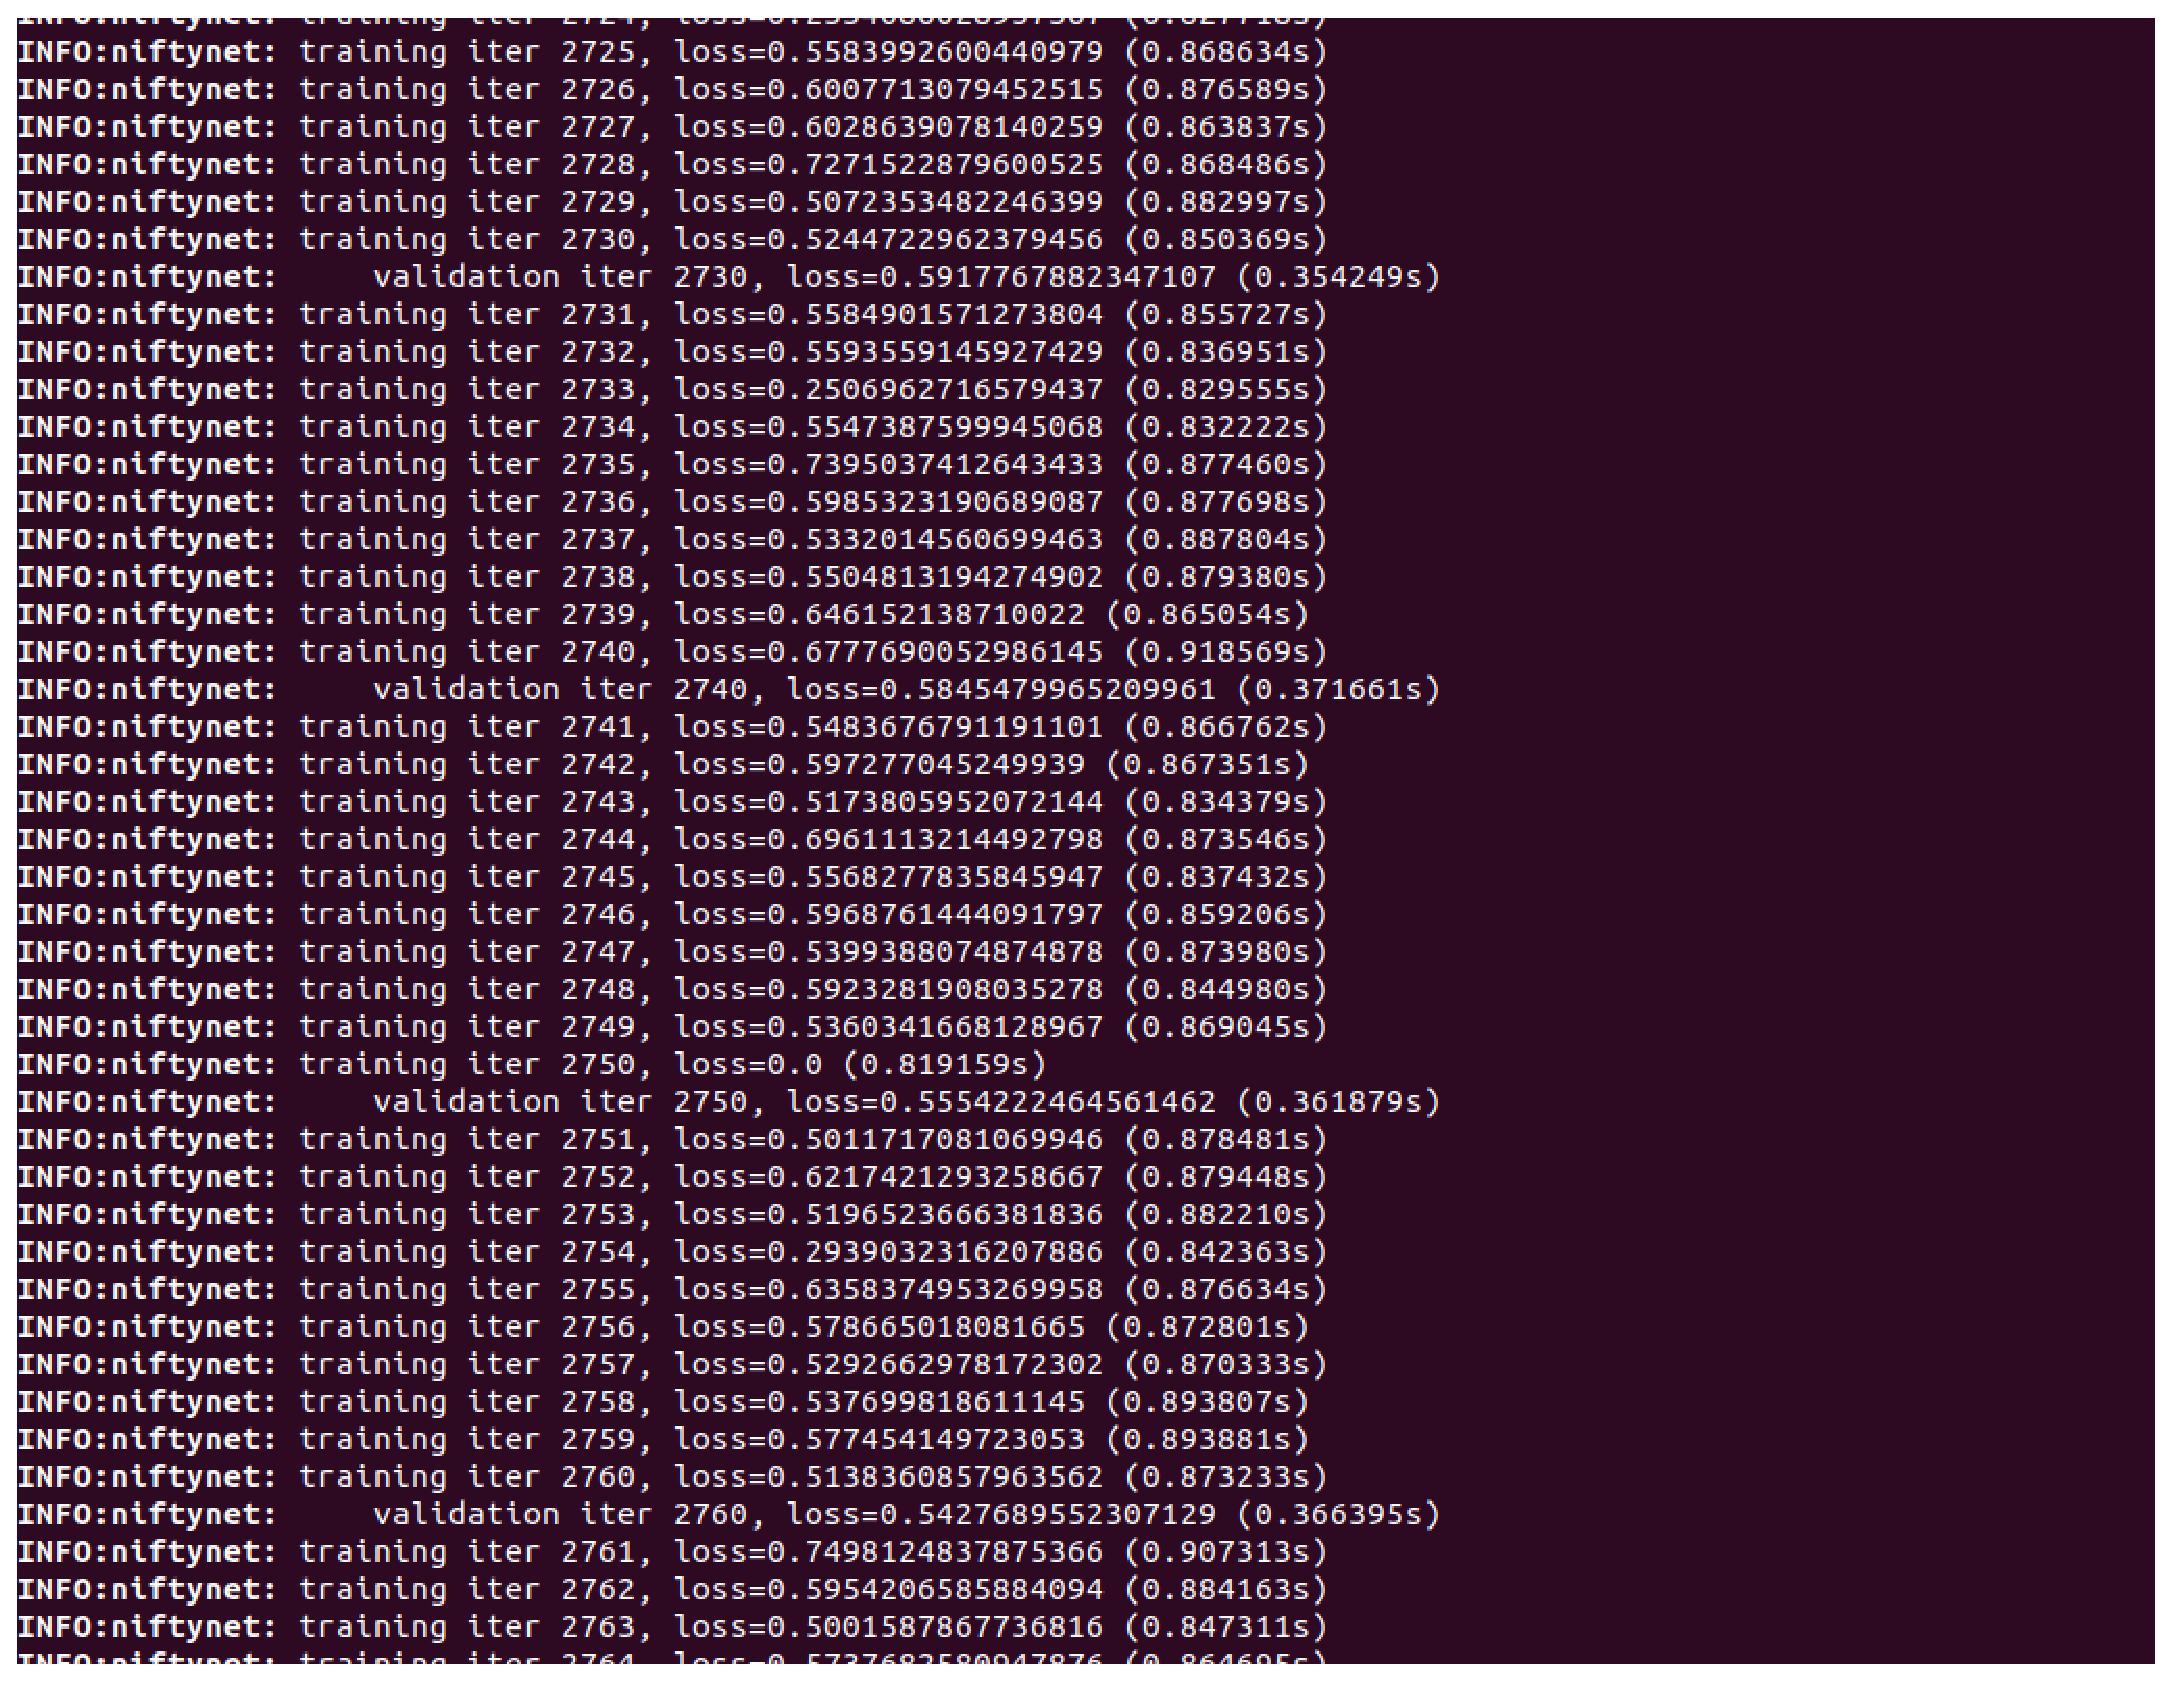
\includegraphics[scale=0.2]{annex/entrainement}
      \caption{Entraînement du système}
      \label{entrainement}
    \end{center}
  \end{figure}
\end{frame}
%--- Next Frame ---%

\begin{frame}[t]{Loss Function}
  \begin{columns}
  \begin{column}[T]{0.01\textwidth}
  \end{column}
  \hfill
  \begin{column}[T]{0.5\textwidth}
    \rouge{-- training}
  \end{column}
  \begin{column}[T]{0.5\textwidth}
    \textcolor{cyan}{-- validation}
  \end{column}
  \end{columns}

  \begin{onlyenv}<1>
    \begin{figure}
      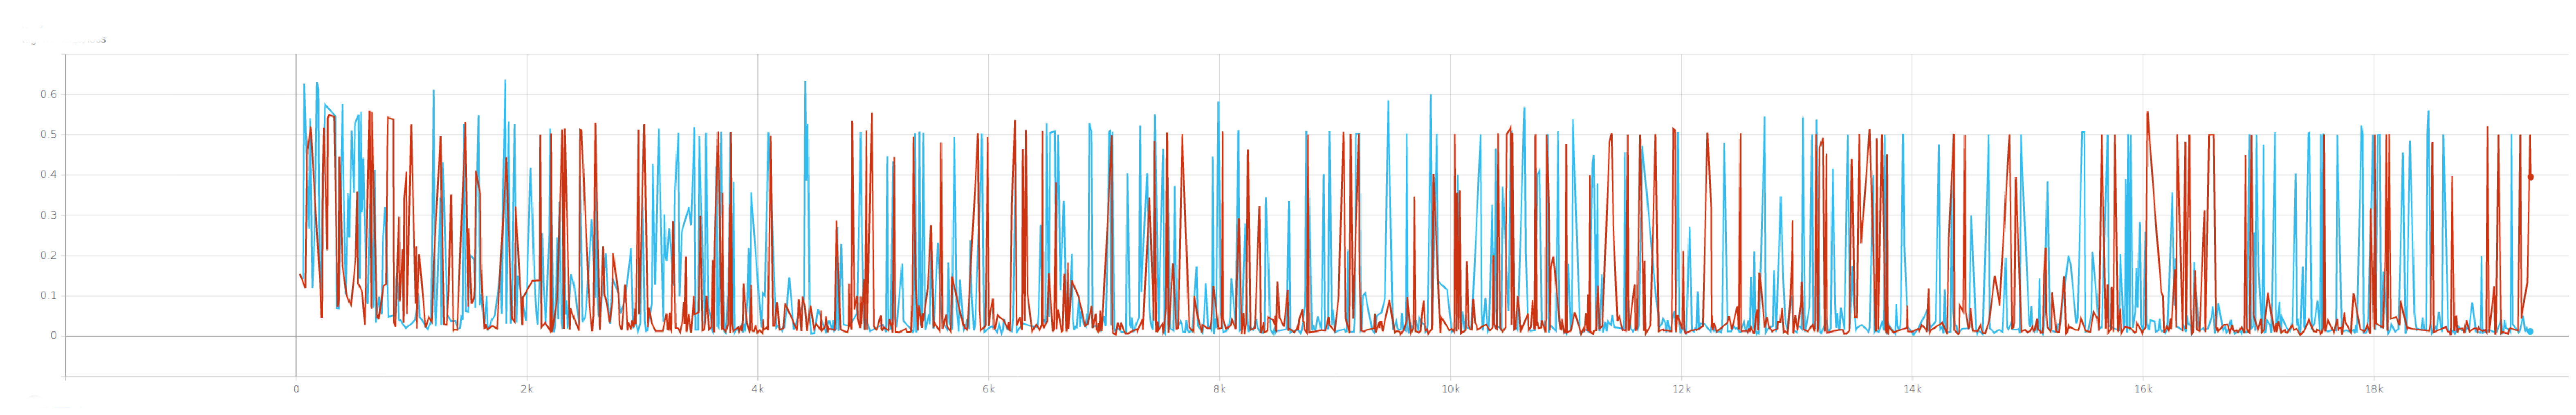
\includegraphics[width=10cm, height=5cm]{annex/loss_not_smoothed}
      \caption{Courbe réelle}
      \label{courbe}
    \end{figure}
  \end{onlyenv}
  \begin{onlyenv}<2>
    \begin{figure}
      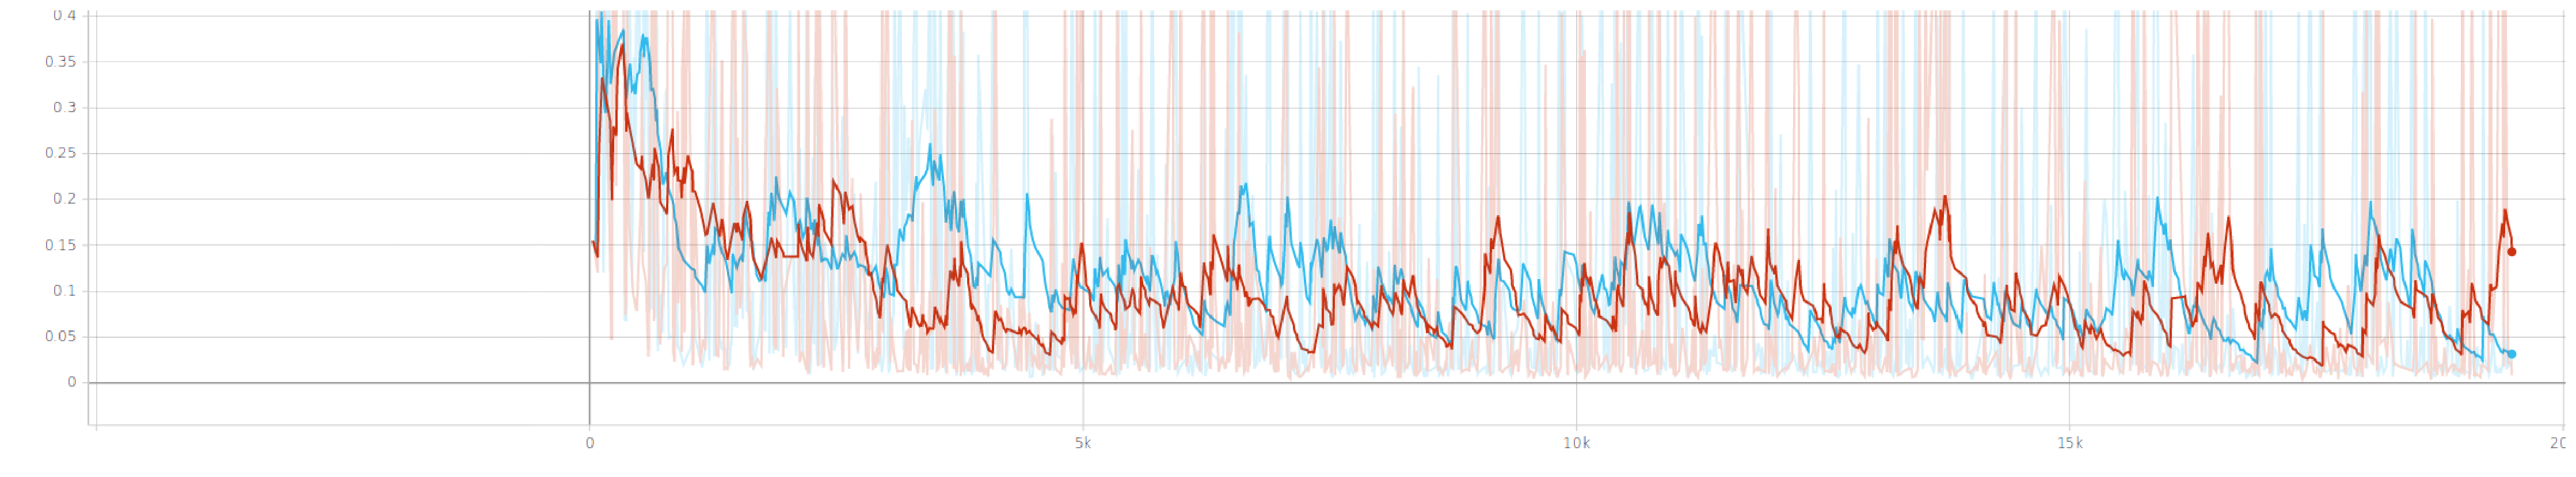
\includegraphics[width=10cm, height=5cm]{annex/loss_smoothed_09}
      \caption{Courbe amortie avec un coefficient 0.9}
      \label{courbe}
    \end{figure}
  \end{onlyenv}
  \begin{onlyenv}<3>
    \begin{figure}
      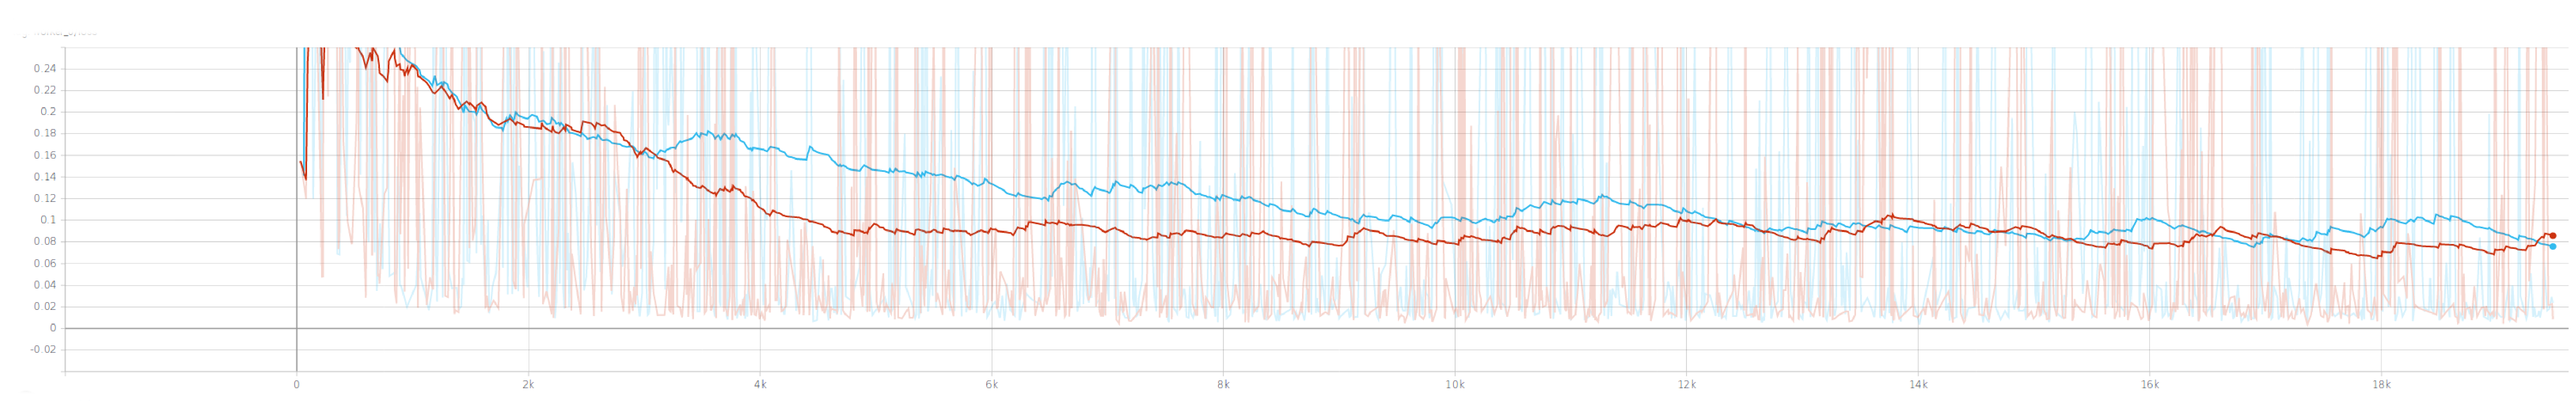
\includegraphics[width=10cm, height=5cm]{annex/loss_smoothed_099}
      \caption{Courbe amortie avec un coefficient 0.99}
      \label{courbe99}
    \end{figure}
  \end{onlyenv}
  \begin{onlyenv}<4>
    \begin{figure}
      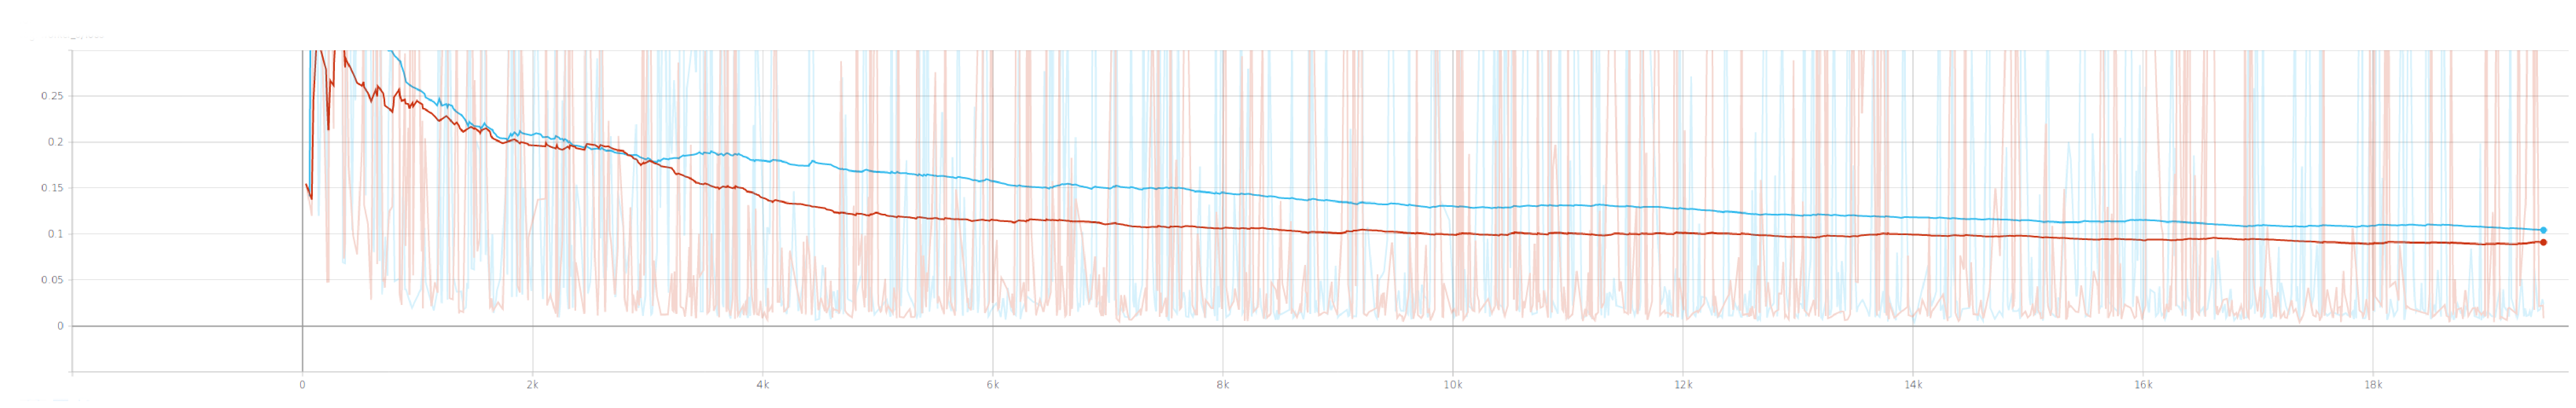
\includegraphics[width=10cm, height=5cm]{annex/loss_smoothed_0999}
      \caption{Courbe amortie avec un coefficient 0.999}
      \label{courbe999}
    \end{figure}
  \end{onlyenv}
\end{frame}
%--- Next Frame ---%

\begin{frame}[t]{Résultats}
  \begin{figure}
    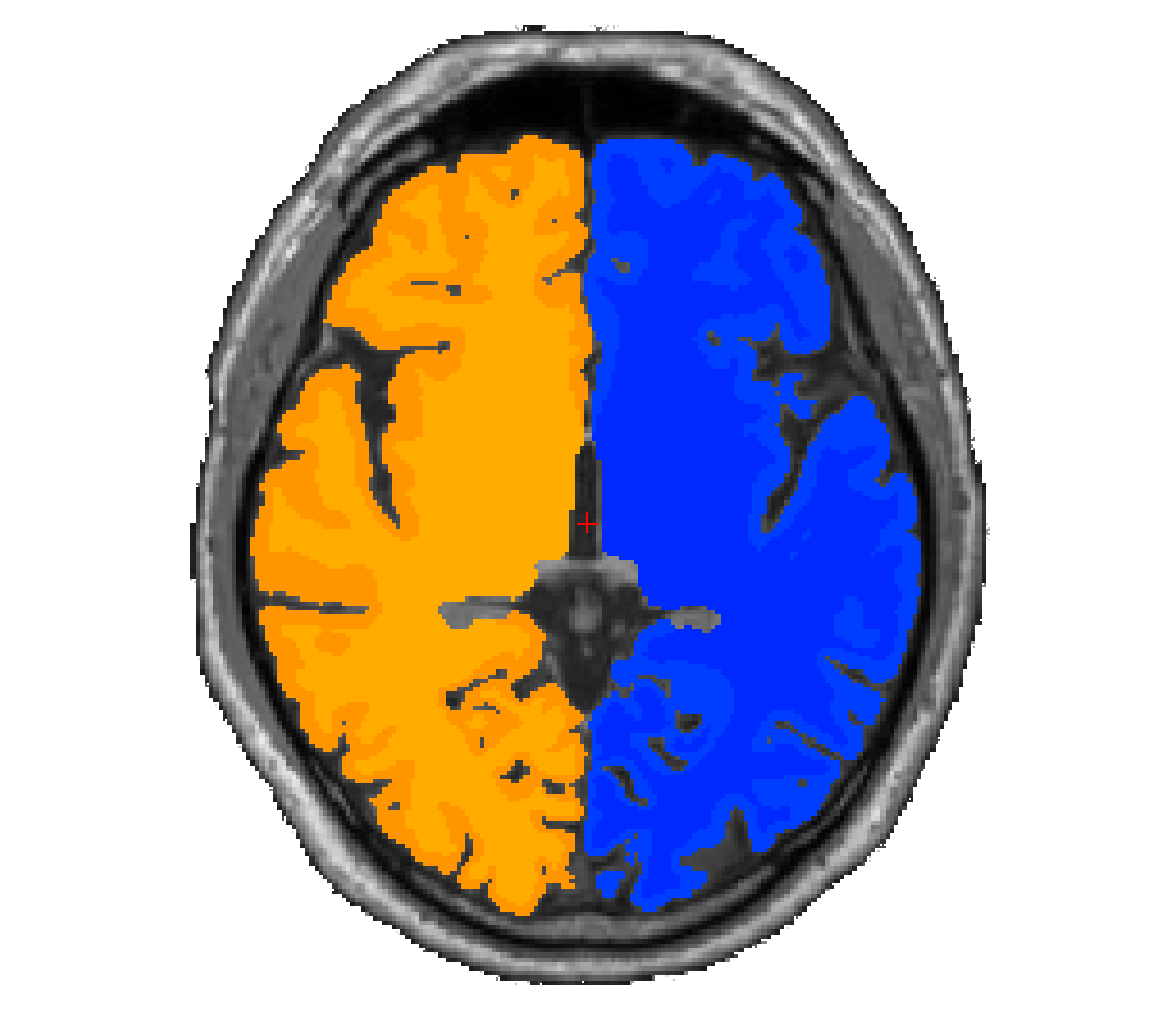
\includegraphics[scale=0.3]{annex/segmentation}
    \caption{Segmentation}
    \label{seg}
  \end{figure}
\end{frame}
%--- Next Frame ---%

\section{Travail à réaliser}

\subsection*{}

\begin{frame}[t]{\'Etude de l'impact du paramètre lr}
  \begin{onlyenv}<1>
    \begin{itemize}
      \item[] \'Etude réalisée avec 2 ``learning rate'' différents :
      \begin{enumerate}
        \item lr = $10^{-3}$
        \item lr = $10^{-6}$
      \end{enumerate}
    \end{itemize}
  \end{onlyenv}
  \begin{onlyenv}<2>
    \begin{figure}
      \begin{center}
        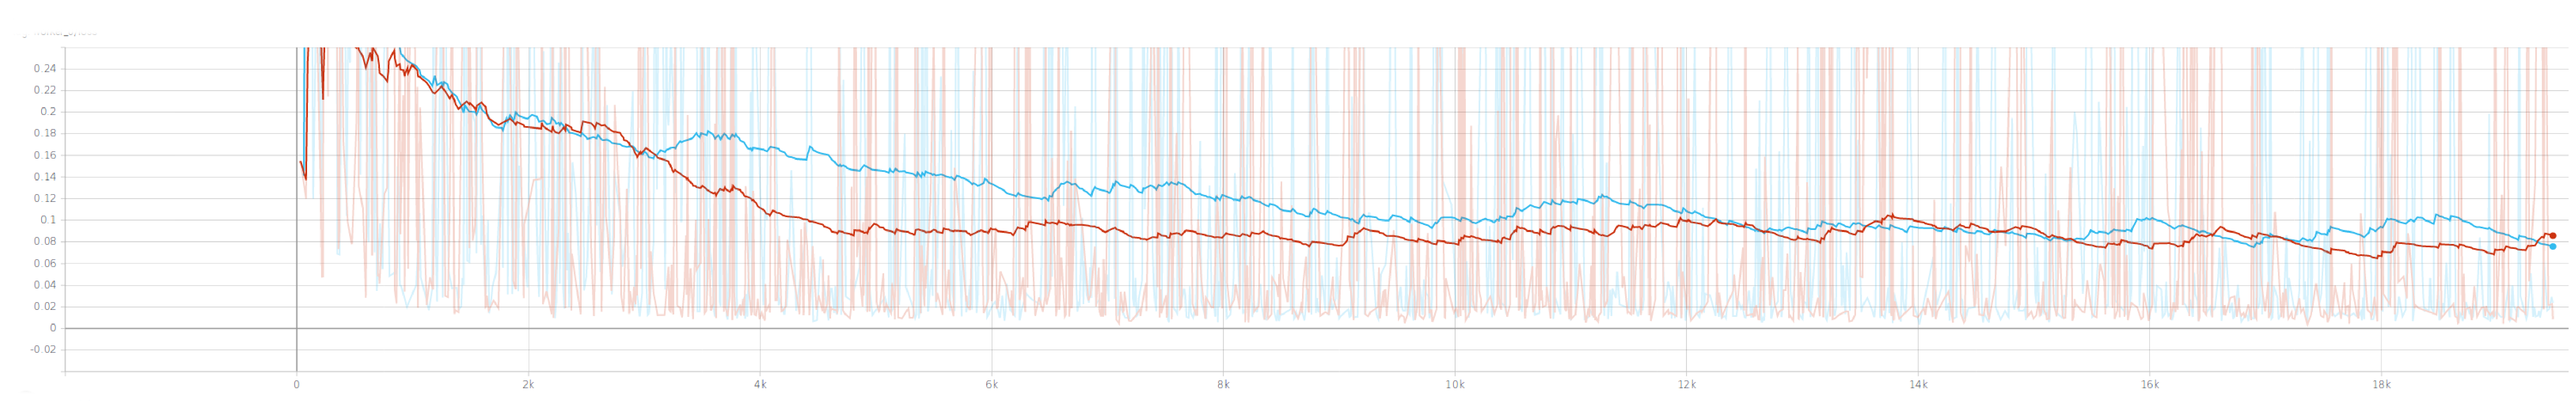
\includegraphics[width=10cm, height=5cm]{annex/loss_smoothed_099}
        \caption{loss function with a learning rate of $10^{-3}$}
        \label{1e3}
      \end{center}
    \end{figure}
  \end{onlyenv}
  \begin{onlyenv}<3>
    \begin{figure}
      \begin{center}
        % 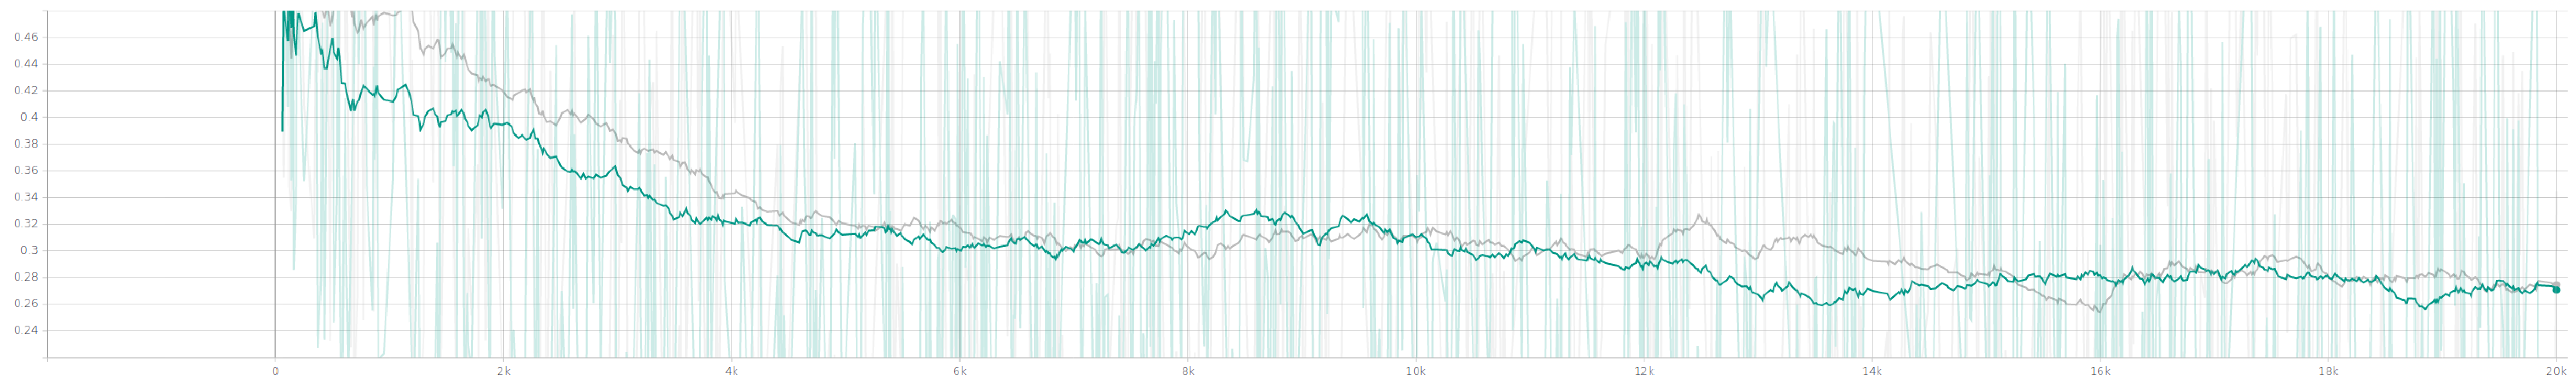
\includegraphics[width=10cm, height=5cm]{annex/loss_1e6}
        \caption{loss function with a learning rate of $10^{-6}$}
        \label{1e6}
      \end{center}
    \end{figure}
  \end{onlyenv}
\end{frame}
%--- Next Frame ---%

\begin{frame}[t]{Première modification du lr}
  \begin{onlyenv}<1>
    \begin{figure}
      \begin{center}
        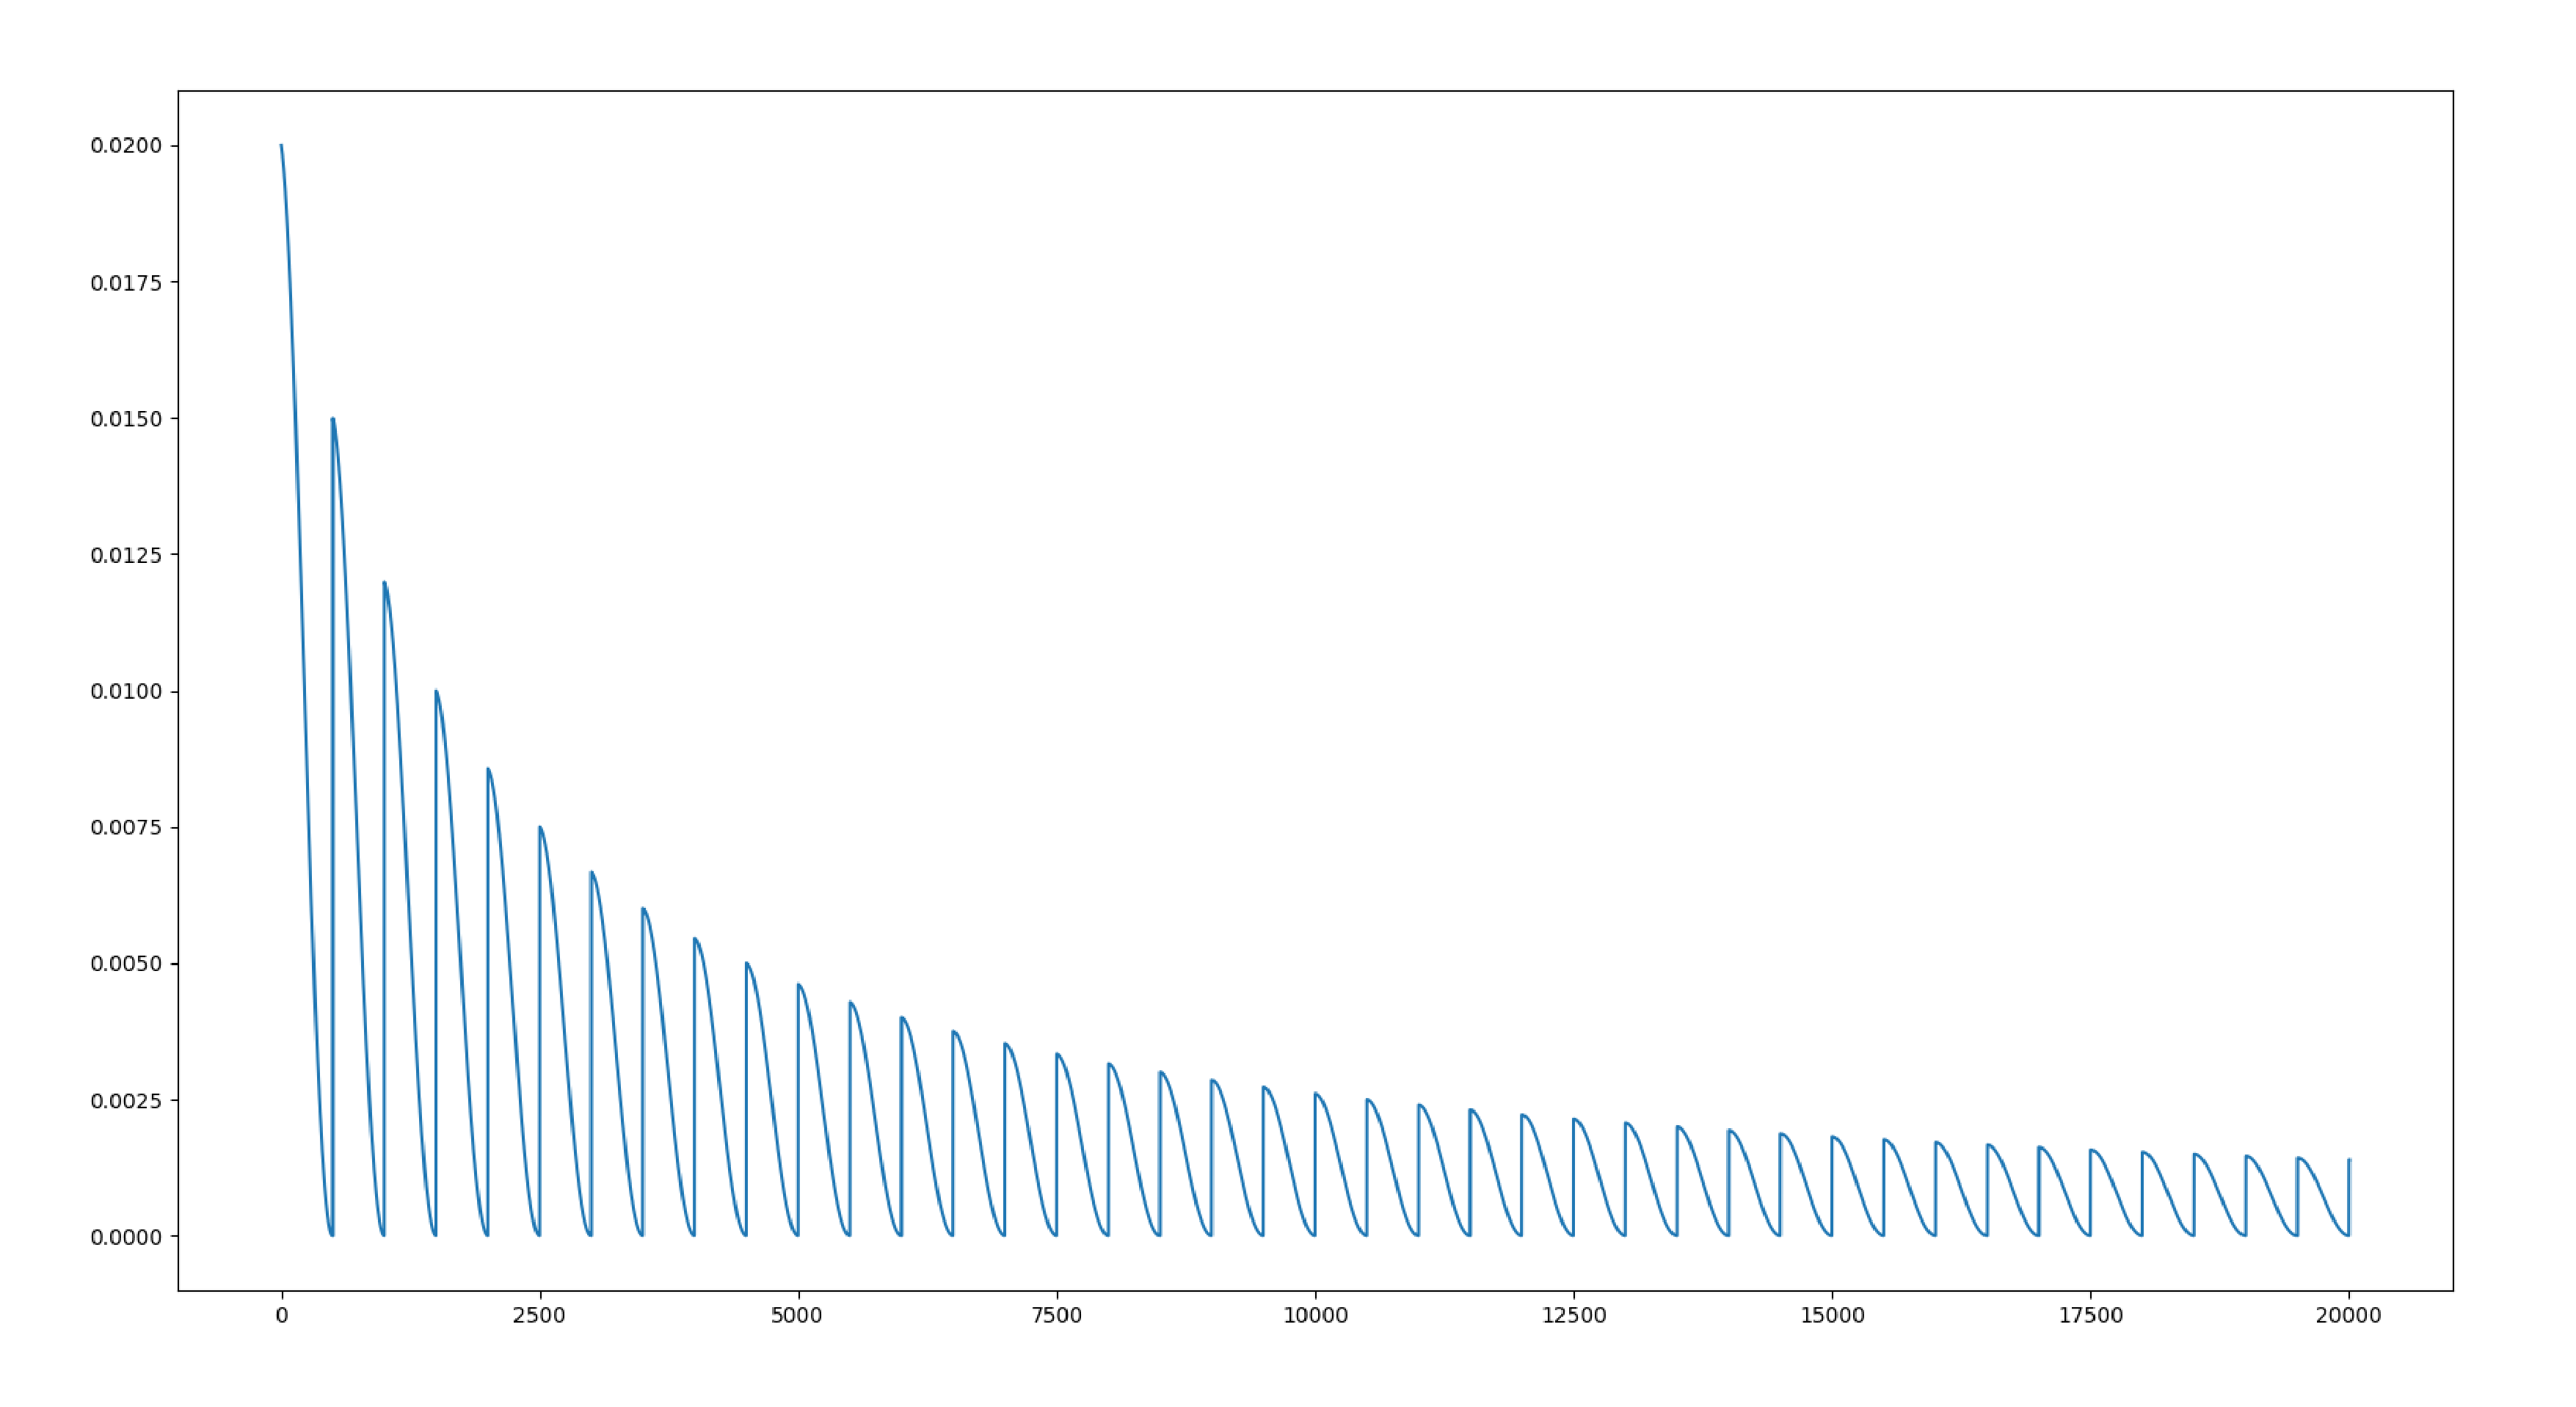
\includegraphics[scale=0.17]{annex/lr_modification}
        \caption{Modification du ``taux d'apprentissage'' à chaque itération}
        \label{ModLR}
      \end{center}
    \end{figure}
  \end{onlyenv}
  \begin{onlyenv}<2>

  \end{onlyenv}
\end{frame}
%--- Next Frame ---%

\section*{Conclusion}

\begin{frame}[t]{Amélioration et Poursuite}
  \begin{itemize}
    \item Modifier le réseau pour de meilleurs résultats
    \item[]
    \item Déterminer le rôle du ``taux d'apprentissage''
    \item[]
    \item Déterminer un algorithme utilisant le ``taux d'apprentissage'' pour optimiser l'apprentissage
  \end{itemize}
\end{frame}

\section*{}

\begin{frame}{Remerciements}
  \begin{beamercolorbox}[ht=2.5ex,dp=1.5ex,center]{frametitle}
    Je vous remercie pour votre attention
  \end{beamercolorbox}
\end{frame}

\appendix

\section*{Annexe}

\end{document}
